\documentclass[a4paper,11pt, twocolumn]{article}
\usepackage[big]{layaureo}
\usepackage[T1]{fontenc}
\usepackage[utf8]{inputenc}
%\usepackage[italian] {babel}
\usepackage{textcomp}
\usepackage{paracol}
\usepackage{amsmath}
\usepackage{authblk}
\usepackage{bbold}
\usepackage{amssymb}
\usepackage{graphicx}
\usepackage{dblfloatfix}
\usepackage{multirow}
\usepackage{caption}
  \captionsetup{format=plain,labelfont=bf,textfont=it, font=small}
\usepackage{subcaption}
  \captionsetup[sub]{position=top}
  \captionsetup[sub]{font=footnotesize}
  \captionsetup[sub]{labelfont={bf,sc}}
\usepackage{booktabs}
\usepackage{longtable}
\usepackage{tabularx}
\usepackage{siunitx}
\usepackage{color}
\usepackage{multicol}
\usepackage{xcolor}
\usepackage{float}
\usepackage{comment}
\usepackage{verbatim}
\usepackage{listings}
\usepackage{physics}
\usepackage{titling}
\usepackage{fancyhdr} %for headers and footers
\usepackage{url}
\def\UrlBreaks{\do\/\do-}
\usepackage{breakurl}
\usepackage[breaklinks]{hyperref}

\newcommand{\subtitle}[1]{%
  \posttitle{%
    \par\end{center}
    \begin{center}\LARGE#1\end{center}
    \vskip0.5em}%
}


\pagestyle{fancy}
\lhead{}
\chead{Life Data Epidemiology}
\rhead{}
\lfoot{Agostini, Bottaro, Pompeo}
\cfoot{}
\rfoot{Page \thepage}
\renewcommand{\headrulewidth}{0.4pt}
\renewcommand{\footrulewidth}{0.4pt}



\title{\textbf{Life Data Epidemiology
\\ \large Study of the influence of the time structure in a network 
for sexually transmitted diseases spreading and vaccination}}

\begin{comment}
Possible titles
+ Study of dynamic network structures in both spreading and vaccination strategies for sexually-transmitted diseases in an online-prostitution community

+ Study of the influence of temporal network structures in spreading and vaccination strategies for sexually-transmitted diseases [MAIN]


\end{comment}{}


\newcommand*\samethanks[1][\value{footnote}]{\footnotemark[#1]}
\author{F. Agostini\thanks{Master Degree in Physics of Data, University of Padua, Italy}, \ \ \ F. Bottaro\samethanks, \ \ \ G. Pompeo\samethanks}


\date{\today}



\begin{document}


%\maketitle
\twocolumn[
  \begin{@twocolumnfalse}
    \maketitle

    \begin{abstract}
    \emph{Context} -- In 2010, Rocha et al. performed studies with data retrieved from an Internet community of clients and prostitutes \cite{rocha}, obtaining information about contacts between nodes and the times they occurred. 

   \emph{Aims} -- In this paper, we will adopt an epidemiologic perspective with the aim to characterize such network and to understand how deeply the time dimension impacts our results, especially in terms of disease prevention.

   \emph{Methods} -- The studies regarding the network will be conducted on two levels, comparing the static aggregate network with the dynamic ones obtained at different time intervals. Simulations will be then implemented to study the diffusion of epidemics onto the two models, particularly focusing on understanding what the most effective vaccination strategies are.
   
   \emph{Results} - We show that the time dimension enriches the modeling capabilities of our network and it implies a greater deal of complexity both in its representation and in the evaluation of its effects. The sparseness of our dataset, however, constituted an obstacle in a profitable data analysis.

    \end{abstract}
    
    {\bf Keywords:} time-dependent networks --
            network spreading --
            SIR model -- 
            vaccination strategies --
            STDs
    \begin{center}
    \rule{0.98\textwidth}{.2pt}
    \end{center}

  \end{@twocolumnfalse}
  
]

{
\renewcommand{\thefootnote}%
    {\fnsymbol{footnote}}
  \footnotetext[1]{Master Degree in Physics of Data, University of Padua, Italy}
}

\section{Introduction}
Computational epidemiology has benefited from the permeation with network science, which allows a rather more realistic way to build models and especially to perform simulations of spreading. However, incorporating a time dimension to a network has often proven to be a challenging task, both from a computational and from a purely representational standpoint.

In this paper, we wish to study the influence of the network structure in the spreading of sexually transmitted diseases (STDs) \cite{stds}. These kinds of diseases are expected to be a common plague within a community of Internet-mediated prostitution. We will hence simulate spreading employing the two most basic compartmental models (SIR and SIS - the SI model is seen just as a particular case of a SIR with $\mu \rightarrow 0$) to analyze how the epidemiologic aspect is influenced by the topology of the network.

Furthermore, we will study vaccination techniques to prevent spreading from happening. To do so, we will particularly focus on the time-dependent network\footnote{While it is true that a temporal network is in fact an ensemble of several, properly-ordered networks, we will often refer to it as a whole, therefore using the singular collective \emph{temporal network}.}, which appears to be a less explored scenario in literature. Moreover, time-dependent networks approximate reality more closely, so the results obtained from them might have a more immediate, practical application.

Because we decide to focus our studies on the network structures, we will disregard the bipartite nature of the network itself. This decision is also supported by the fact that most STDs do not appear to have a significantly different incidence ratio between male and female populations, at least for the matters we are mostly concerned with \cite{stds_inc}.  


\section{Methodology}
\subsection{Code development}
Our code for analysis was developed in \emph{Python}. In particular, two packages were employed to perform the core network analyses and the simulations on them.

The \texttt{networkX} package \cite{networkx} is a package for the creation, manipulation and study of the structure, dynamics, and functions of complex networks. We mainly employ it to characterize the properties of the networks we are working with (both the aggregate one and the temporal sequences) and to manipulate them, for example through node or link removals when implementing vaccination strategies.

The \texttt{EoN} package (\texttt{Epidemics on Networks}) \cite{simulations} is instead the one dedicated to epidemiologic simulations on networks: for our purposes, it allows to carry out stochastic simulations of epidemics, with custom-built functions for both SIR and SIS model. These tools greatly outperform even a Gillespie algorithm by means of \emph{synchronous update} and they work under suitable assumptions for our study case (i.e.: exponentially distributed infection and recovery times).


\subsection{Static network}
At first, we opt to study the \emph{aggregate static network}, obtained from the combination of all the intervals of the time-dependent network. After obtaining a general overview of the network properties, we perform a \emph{grid search} in the $\beta - \mu$ space parameter; this is done in a range which is broad enough for us to understand how prone the network is to epidemic spreading, but also such that it is focused enough in a sensible order of magnitude for the kinds of diseases we are considering. According to each case, we will be considering the values $s_{\infty}$, $x_{\infty}$ and $r_{\infty}$, respectively fractions of susceptibles, infected and recovered at equilibrium, in order to establish whether a spreading occurred or not. We will do so both for a SIR and a SIS model, with an assigned number of initial infected randomly distributed over the aggregate network.

Vaccination strategies will then be implemented by targeting the \emph{superspreaders}, meaning the hubs. In our specific context, these hubs are represented by the most sexually active prostitutes and/or clients, which are the most exposed victims of STDs due to their high number of contacts. 


\subsection{Temporal network}
The time dimension introduces another level of complexity altogether, as already noted for example in \cite{sir_net}. We again need to retrieve the properties of the underlying network, which is done by building a list with the first node of each link, one with the second one and a list with the time in which each link is active. 

It should be noted right away that we decide to combine the time information in intervals of $\Delta t = 30$ days, meaning that we have a 30-day time resolution: this will prevent transient effects from disrupting significantly our analysis and will partially smooth out the extreme sparseness of our network. Furthermore, to expand our dataset, we impose periodical conditions: after the final day, our timeline will restart back at day $1500$ (this is done to exclude spurious effects when the community is not fully operational).

The time dimension offers an insight in the evolution of the Internet community over the months and it makes it possible to assess the different behaviours that take place among its members. This, while implicating higher complexity, definitely offers a more loyal representation of reality.

Again, simulations of disease spreading are then performed with the two main compartmental models. In this scenario, we can take advantage of the time dimension by allowing the newly-entered nodes (as previously mentioned, we disregard whether they are prostitutes or clients) to be infected with probability $p = 0.001$. We also carry out simulations as before and compare the two results.

%   qui sotto è tutto parziale: "parte creativa"
%   RICONTROLLARE 
\subsection{Manipulative analysis on temporal network}
To fully exploit the time information we have at disposal, we broaden our analysis introducing some variations in our dataset. We wish to artificially create circumstances for an easier spreading of the diseases by altering the network both spatially and chronologically, hence losing, from now on, the connection with the real community described by the data.

To begin with, we will implement Random Reference Models (RRMs), in order to compare the epidemics effects on real data with the outcome in appropriate null models and validate the results. We will obtain such new networks by means of global node or time-interval shuffling: in the former case, we shuffle the node labels, hence altering the connections that in fact take place between individuals; the latter approach modifies the time structure, rearranging the instants at which contacts occur.

In addition to that, in order to focus on the most active nodes, we study the subcommunity of those people who had at least 5 contacts, for example imagining that the subscription to the Internet forum demands a minimum number of interactions for the online profile to be kept active, limiting the presence of \emph{bystanders} or casual visitors in the community. 


\section{Results}
\subsection{Static network}
In the aggregate network we have all the links present at once, so we can build a node degree distribution, albeit not representing any our system is ever actually in.
\begin{figure}[H]
\centering
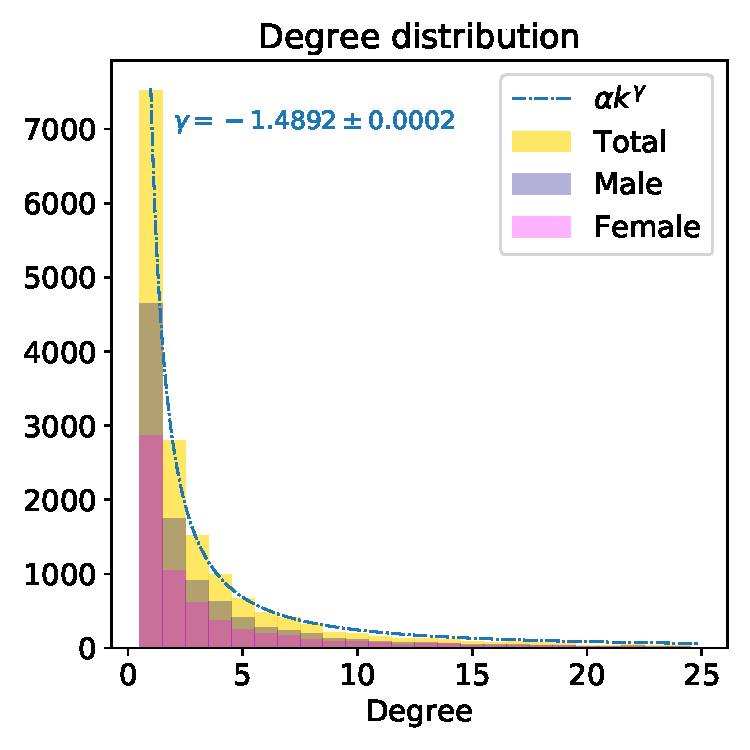
\includegraphics[scale=0.3]{./Figure/Static/Degree_distribution.pdf}
\caption{Node degree distribution for the aggregate network, with distinction between male and female}
\end{figure}
The distribution follows a clear power law, with exponent $\gamma = -1.4892 \pm 0.0002 $.
The total number of connected components is 
\begin{center}
    $N_{connected} = 418$
\end{center}{}
which signals an incredibly sparse network, all in all a foreseeable aspect considering the huge amount of nodes with very few activations. This will likely result in little permeability from the network to disease spreading.

\subsubsection*{Simulations}
\begin{figure*}[t!]
\begin{subfigure}[t]{0.32\textwidth}
\centering
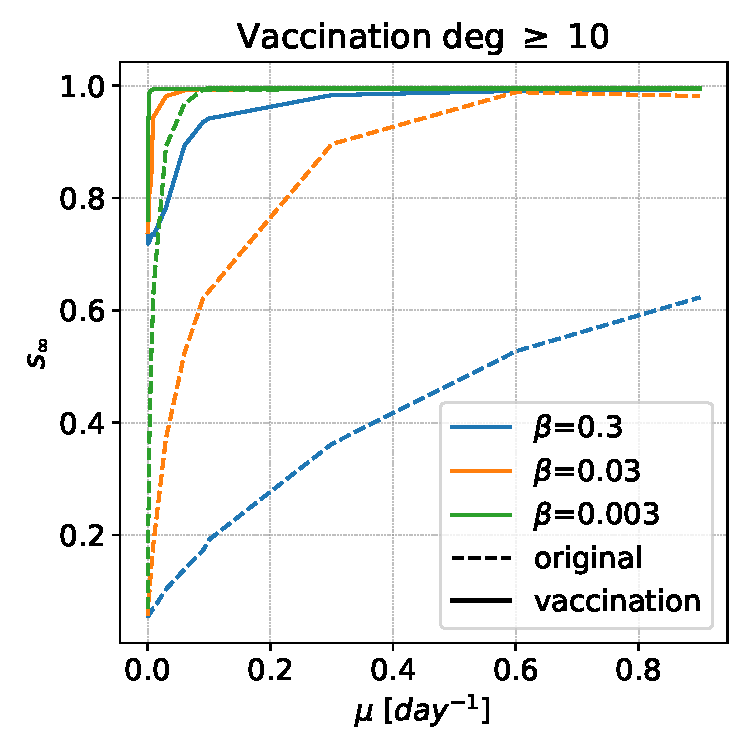
\includegraphics[scale=0.30]{./Figure/SIR/vax_deg_10.pdf}
\caption{}
\end{subfigure}
\begin{subfigure}[t]{0.32\textwidth}
\centering
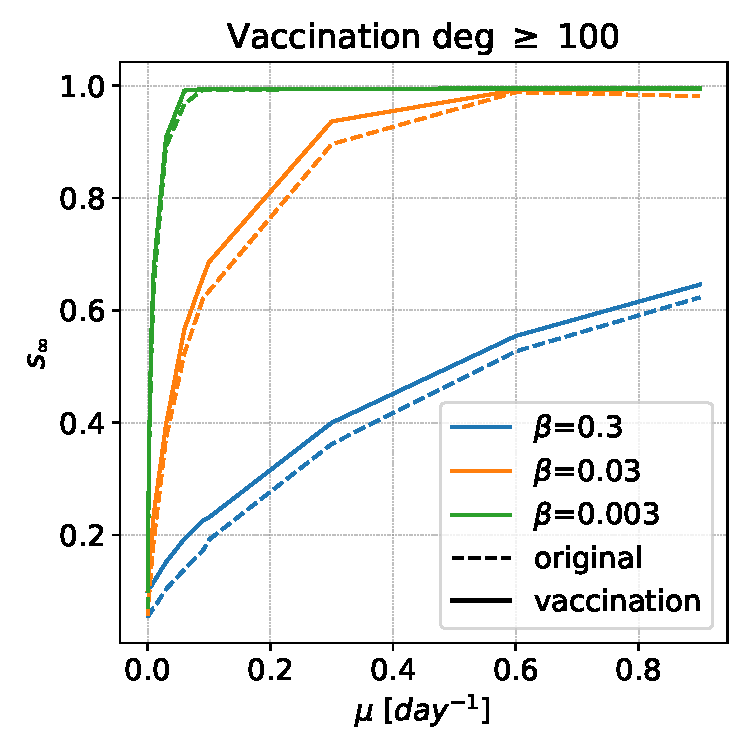
\includegraphics[scale=0.30]{./Figure/SIR/vax_deg_100.pdf}
\caption{}
\end{subfigure}
\begin{subfigure}[t]{0.32\textwidth}
 \centering
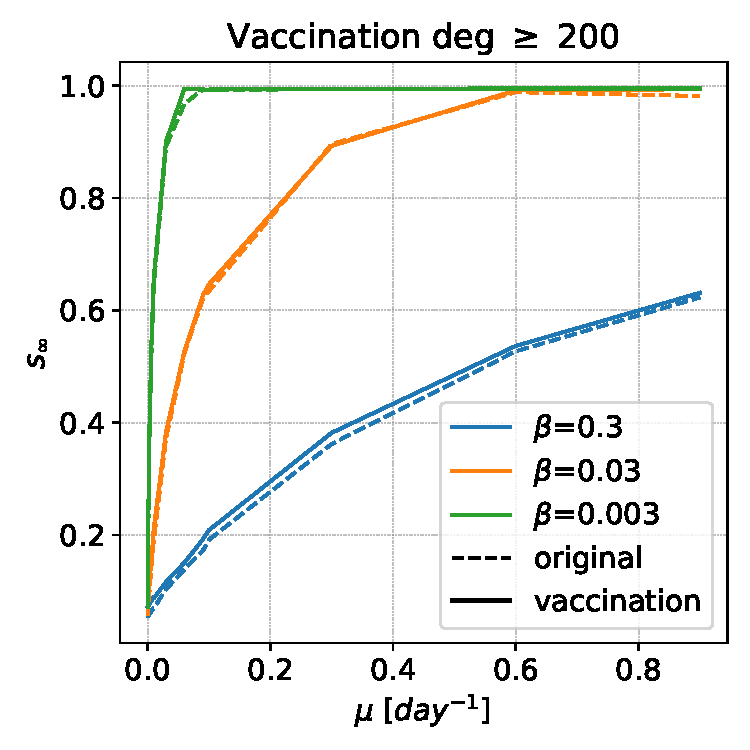
\includegraphics[scale=0.30]{./Figure/SIR/vax_deg_200.pdf}
\caption{}
\end{subfigure}

\begin{subfigure}[t]{0.32\textwidth}
\centering
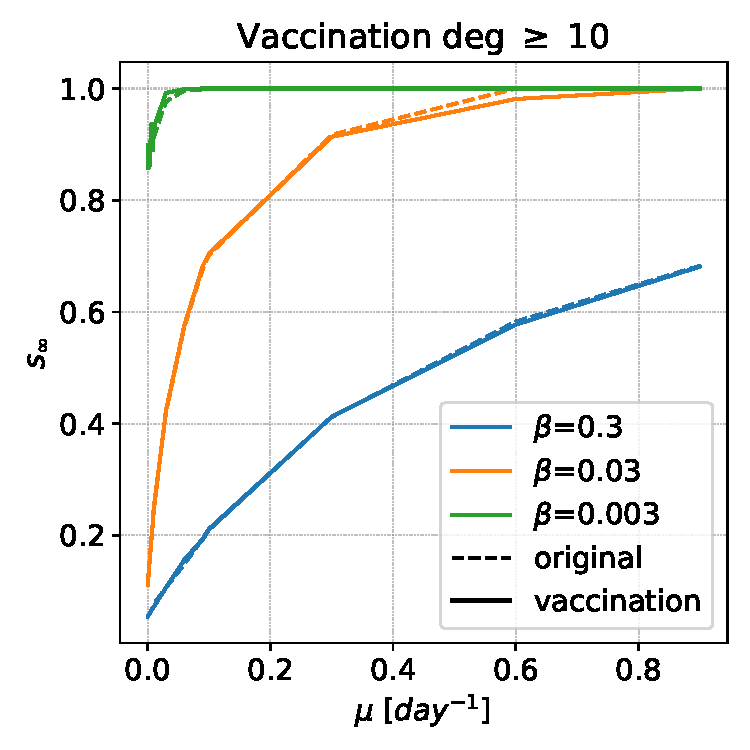
\includegraphics[scale=0.30]{./Figure/SIS/vax_deg_10.pdf}
\caption{}
\end{subfigure}
\begin{subfigure}[t]{0.32\textwidth}
\centering
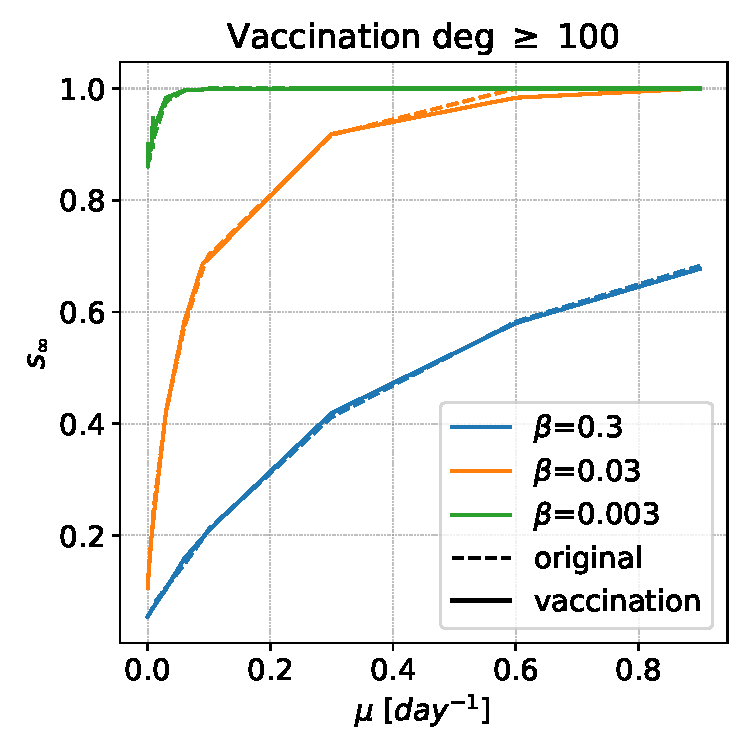
\includegraphics[scale=0.30]{./Figure/SIS/vax_deg_100.pdf}
\caption{}
\end{subfigure}
\begin{subfigure}[t]{0.32\textwidth}
 \centering
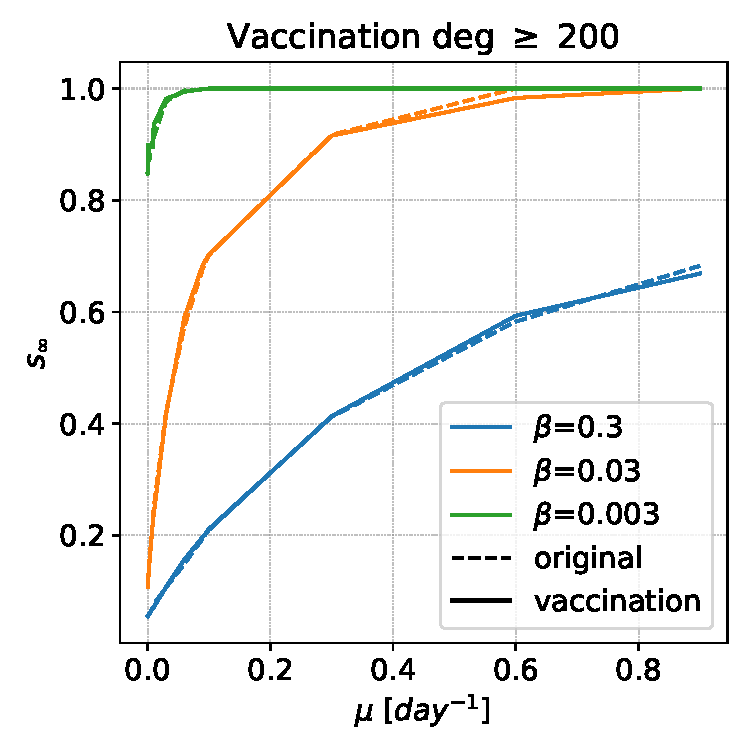
\includegraphics[scale=0.30]{./Figure/SIS/vax_deg_200.pdf}
\caption{}
\end{subfigure}
\caption{Results for the vaccination strategies implemented with an underlying SIR model (Fig. A-C) and SIS model (Fig. D-F). From left to right, the degree of the vaccinated nodes must higher than the threshold declared in the title (10, 100 and 200 respectively).}
\label{static_sims}
\end{figure*}

\begin{figure}[H]
\begin{subfigure}[t]{0.49\textwidth}
\centering
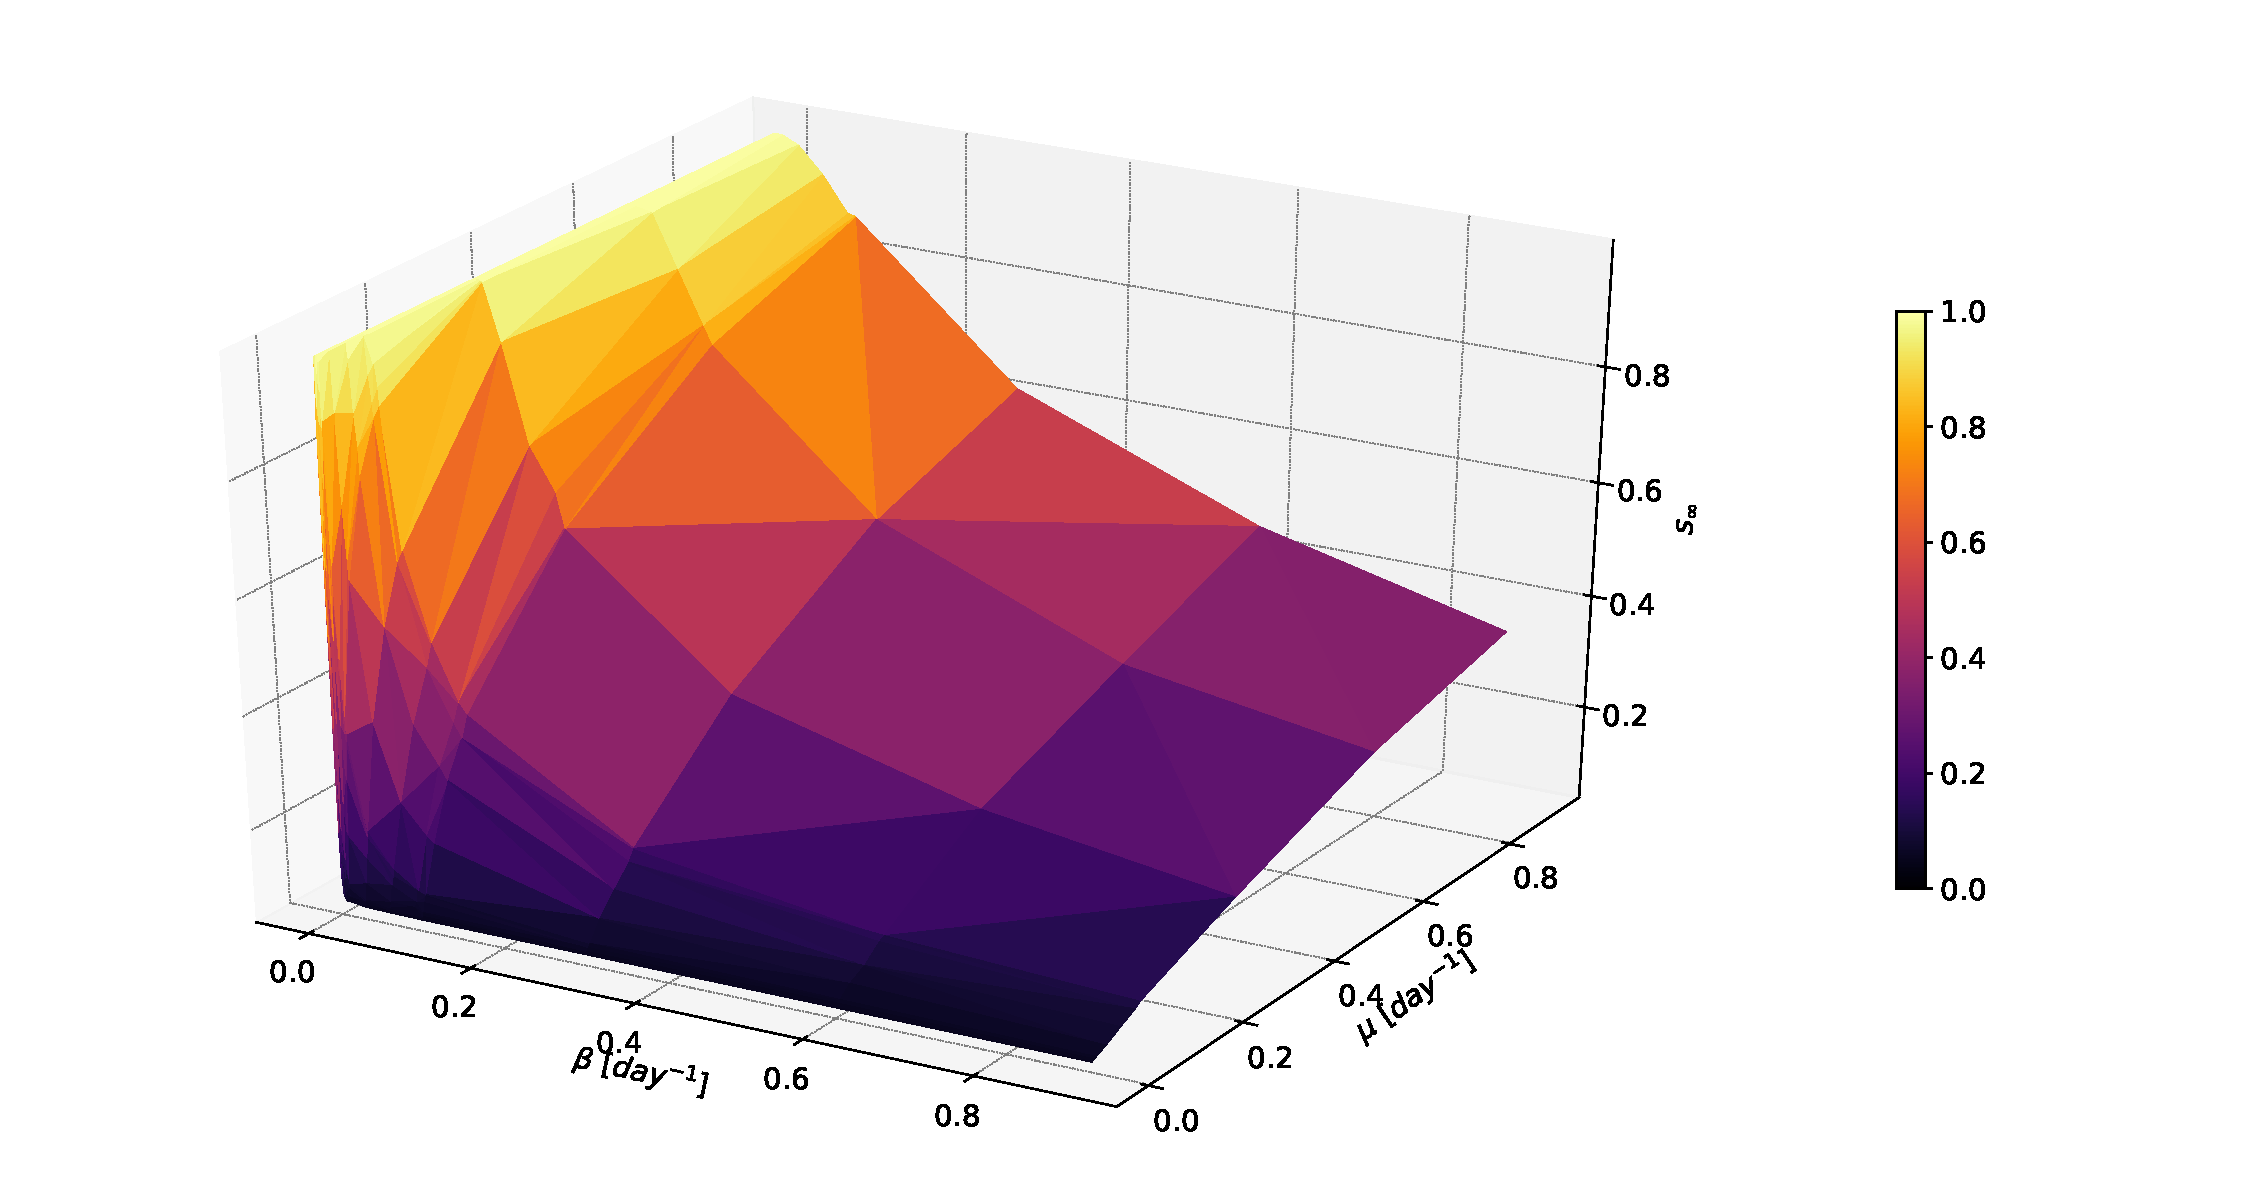
\includegraphics[width=\textwidth]{./Figure/SIR/S_inf_surface.pdf}
\caption{SIR}
\label{grid_SIR}
\end{subfigure}
\begin{subfigure}[t]{0.49\textwidth}
\centering
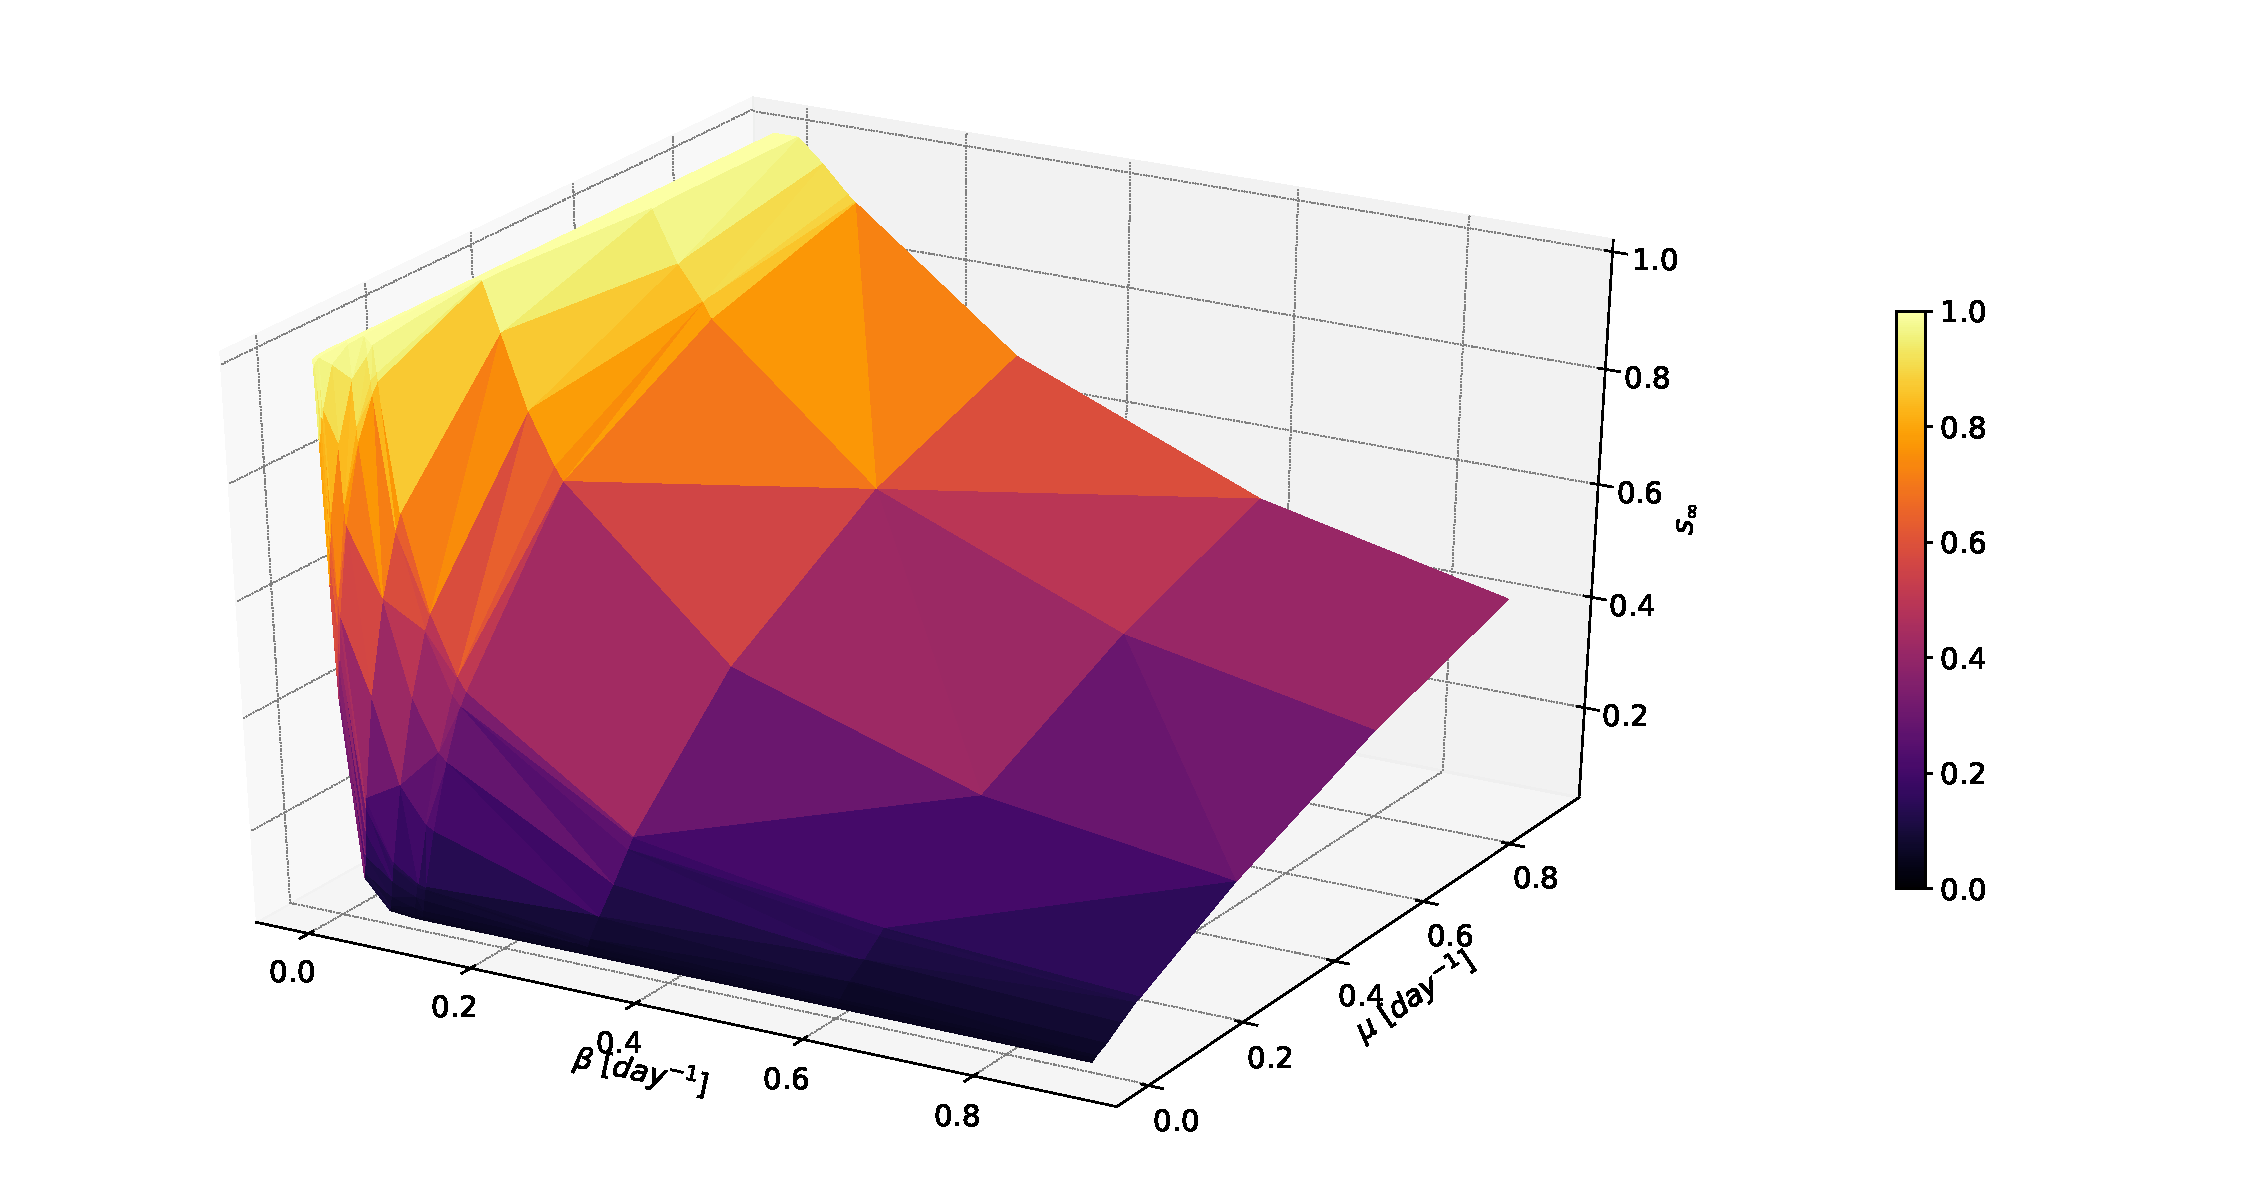
\includegraphics[width=\textwidth]{./Figure/SIS/S_inf_surface.pdf}
\caption{SIS}
\label{grid_SIS}
\end{subfigure}
\caption{3D-surfaces representing the values of $s_{\infty}$, fraction of susceptibles, obtained for the two epidemic models as a function of the parameters $\beta - \mu$ in the portion of space considered for tuning.}
\end{figure}

We consider the two compartmental models, SIR and SIS (this one is actually the most suitable for sexually-transmitted diseases, which hardly cause immunity in patients), and we perform a grid search on the contagion rate $\beta$ and the recovery time $\mu$.

We wish to understand the range of parameters that make it possible for a disease to spread in our network, but we still do so with a focus on the order of magnitude of STDs.

We notice how the aggregate static network does not appear very prone to spreading, but a parameter region can be individuated in both plots where the number of susceptibles is such that it confirms a pathogen has spread in the network.

For the SIR model (Fig. \ref{grid_SIR}), wherever $s_{\infty}$ is null or close to 0, it means that the remaining fraction of nodes has undergone an illness process and they are now either in the infectious or in the recovered state. As far as SIS is concerned (Fig. \ref{grid_SIS}), we remind that $1-s_{\infty}$ is the fraction $x_{\infty}$ of infected individuals, so where the amount of susceptibles is negligible, the number of people who got the disease will be significant.

We therefore move forward implementing \emph{vaccination strategies} in our network, in order to see how effective this kind of operation would be in a static graph.

Overall, in Fig. \ref{static_sims}, we notice how the removal does not change significantly the scenario in either models. Removing the biggest hubs (nodes with degree higher than $200$) has the effect of a simple fluctuation. This somewhat clashes with the network degree being distributed as a power law: our expectation would have been that the removal of the hubs should have caused a greater impact.

The fact that it takes a removal of all the nodes having degree higher or equal to $100$ to distinguish any effect could be due, in our hypothesis, to the extreme sparseness that characterizes the network. The idea is not that the vaccinations are ineffective, rather that it is very hard to influence this kind of structure in any way, unless a drastic policy is pursued.

Also, the effect on the SIS model is much less noticeable because of the absence of a recovery state.

We eventually decided not to implement a random removal strategy considering how little effectiveness even a targeted vaccination has proven to have on our network.



%%%%%%%%%%%%%%%%%%%%%%%%%%%%%%%%%
%%%%%%% TEMPORAL
%%%%%%%%%%%%%%%%%%%%%%%%%%%%%%%%%
\subsection{Temporal network}
In what represents the main focus of our analysis, we start by assessing how the evolution of the community takes place. At this point, we have not aggregated the dataset to a wider time window, nor have we introduced any kind of periodicity yet; moreover, we will momentarily keep the distinctions between males and females, in order to obtain a richer description of the dataset itself.

\begin{figure}[H]
\begin{subfigure}[t]{0.24\textwidth}
\centering
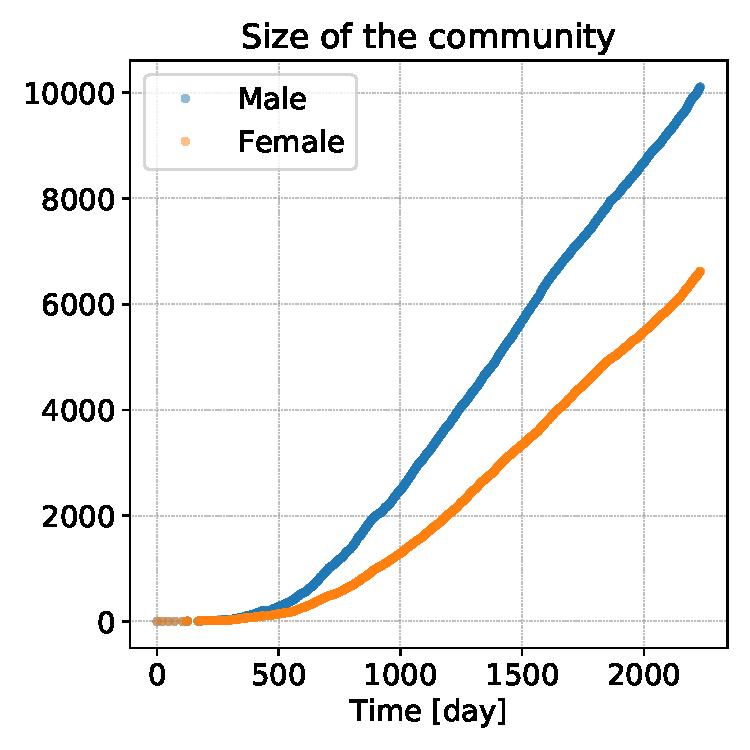
\includegraphics[scale=0.30]{./Figure/Static/Size_community.pdf}
\caption{Cumulative number of nodes partaking in the community over the data period considered.}
\label{growth}
\end{subfigure}
\begin{subfigure}[t]{0.24\textwidth}
 \centering
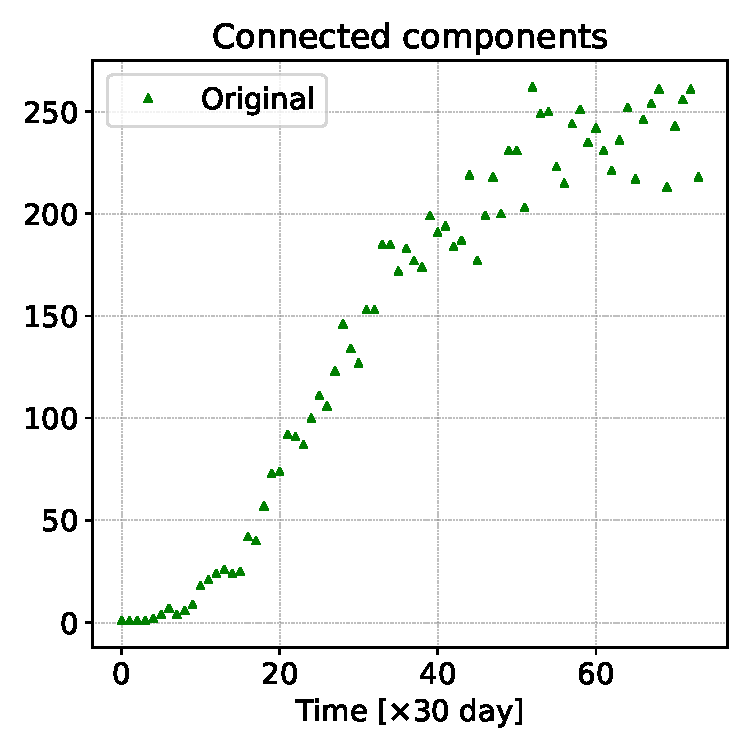
\includegraphics[scale=0.30]{./Figure/Temporal/connected_components_original.pdf}
\caption{Number of connected components in the network at each time-step.}
\end{subfigure}
\caption{}
\end{figure}

It appears that the community is growing, but Fig. \ref{growth} still represents a cumulative plot (therefore connected to the aggregate network, in a way) and it therefore should be taken with care. Time-wise, it is also quite clear how the number of connected components grows in a logistic fashion, following what is a typical trend of growth in an (online) community.

If we consider the activations that each node undergoes at a given time-step, the trend varies significantly, but it still is increasing, generally; we now consider the network evolution both as far as nodes and links are concerned.

\begin{figure}[H]
\begin{subfigure}[t]{0.24\textwidth}
\centering
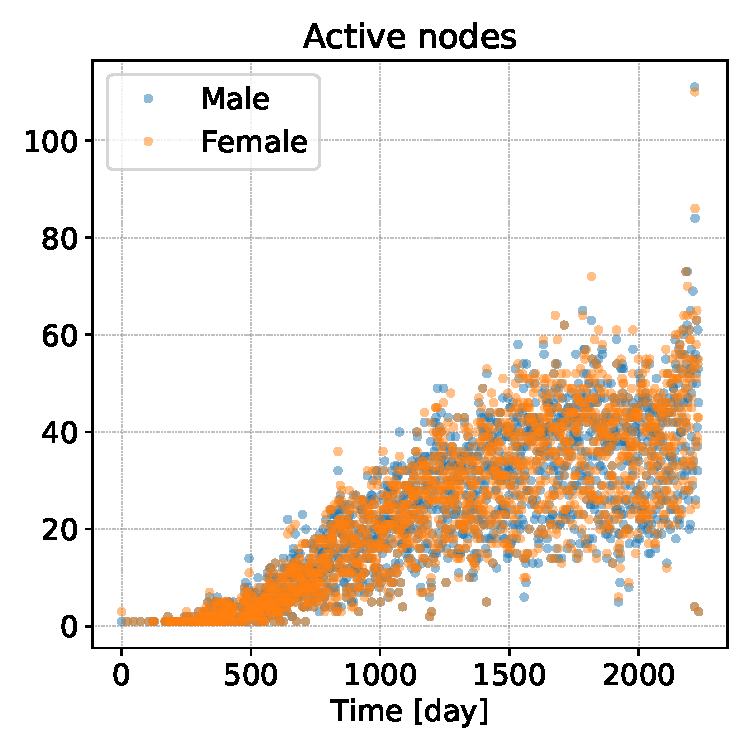
\includegraphics[width=\textwidth]{./Figure/Static/Active_nodes_MF.pdf}
\caption{Number of active nodes at each registered time iteration, with distinction between male and female members of the community.
}
\end{subfigure}
\begin{subfigure}[t]{0.24\textwidth}
 \centering
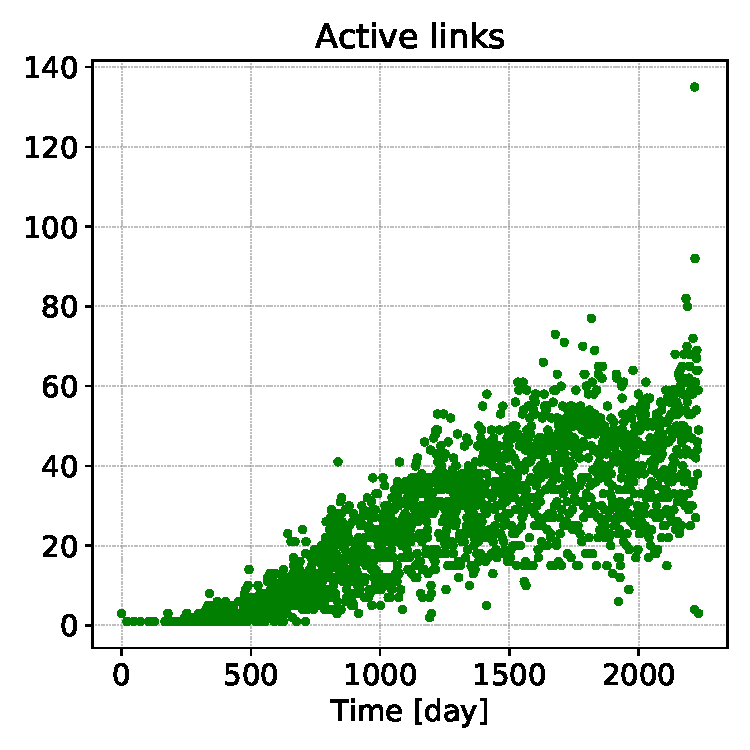
\includegraphics[width=\textwidth]{./Figure/Static/Active_links.pdf}
\caption{Number of active links at each registered time iteration.}
\end{subfigure}
\caption{}
\end{figure}

Once again, even if there are several fluctuations depending on variables we are not accounting for (even the day of the week, as an example, has quite a bit of influence in the frequency of sexual encounters), a general increasing trend can clearly be spotted, both in the nodes (members of the community) and links (connections between the members).

However, if we rather focus on the fraction of active nodes on the total number of participants in the forum at that given time-step, we notice how this value clearly has a downward trend.
\begin{figure}[htp]
\centering
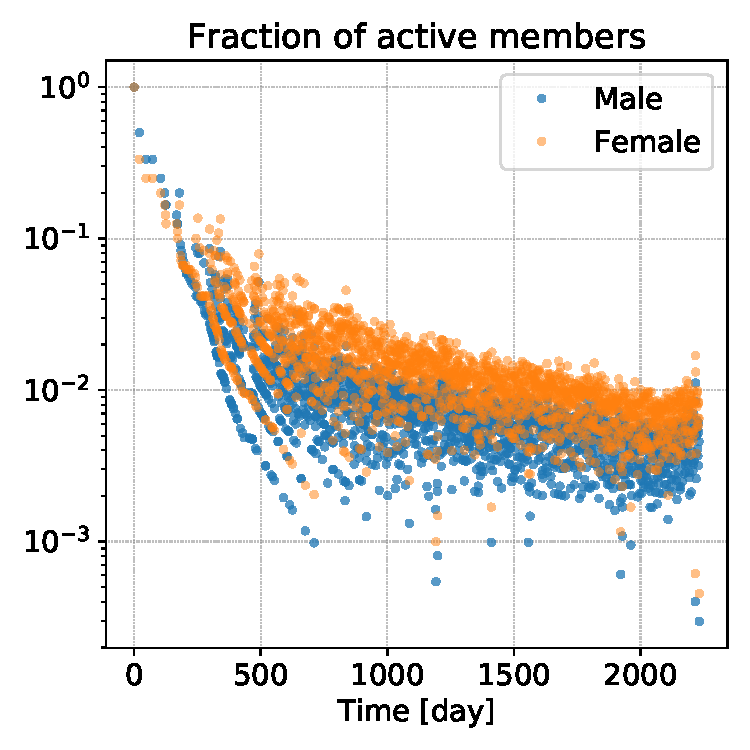
\includegraphics[scale=0.3]{./Figure/Static/Fraction_active_members.pdf}
\caption{Fraction of active members at each time iteration over the total members of the community at that time-step.}
\end{figure}

As already noted in preceding studies (\cite{rocha, internet_pros}), this is typical: we have the very vast majority of nodes undergoing only few -- if not just one -- activations, with very long interactivation times. In practice, there is only a small group of either sex-buyers or sex-sellers who keep themselves active in the community at a fairly constant rate. This is an aspect that will definitely need to be taken into consideration when simulating a possible STD spreading.

\subsubsection*{Simulations}
As with the static aggregated network, we perform the same simulations for the temporal network, employing the same compartmental models, a SIR and a SIS. We remind that this kind of analyses will be performed by aggregating the time sequences into 30-day windows and we will introduce a periodicity in the dataset, forcing it to restart back from week $50$ (hence excluding the first $5/7$ of it, because it shows inconsistent and bursty behavior).

\begin{figure}[H]
\begin{subfigure}[t]{0.49\textwidth}
\centering
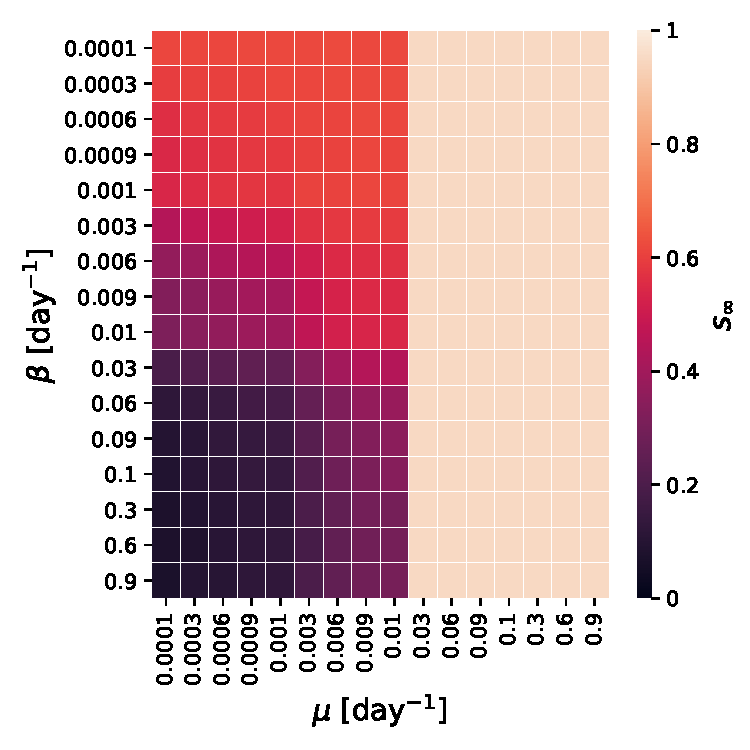
\includegraphics[scale=0.52]{./Figure/Simulations/SIR_temporal_16482.pdf}
\caption{SIR}
\label{grid_SIR_temp}
\end{subfigure}
\begin{subfigure}[t]{0.49\textwidth}
\centering
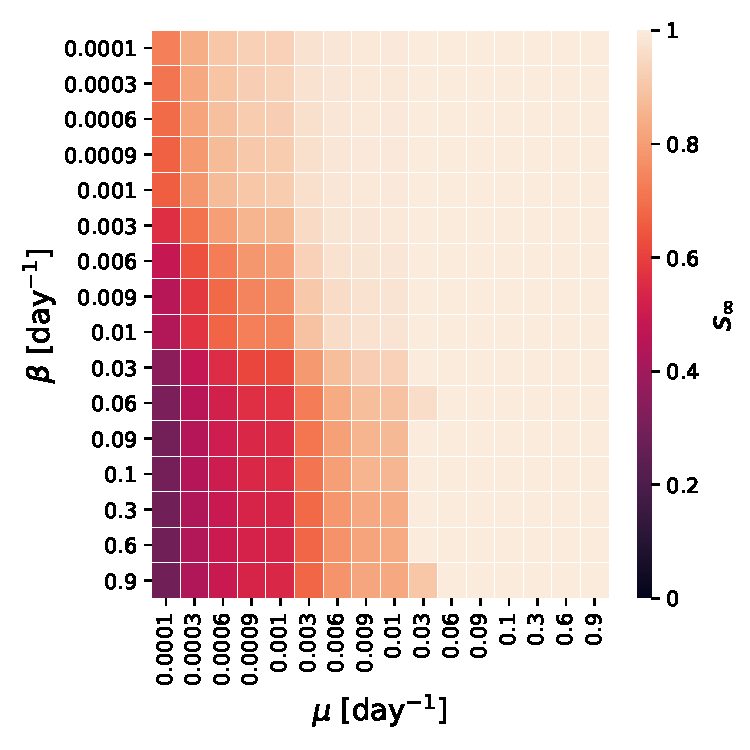
\includegraphics[scale=0.52]{./Figure/Simulations/SIS_temporal_72633.pdf}
\caption{SIS}
\label{grid_SIS_temp}
\end{subfigure}
\caption{Heatmaps representing the fraction $s_{\infty}$ of susceptibles at equilibrium for each combination of parameters $\beta$ and $\mu$. This form of visualization was preferred with temporal networks to better display the phase transition happening for a critical value of recovery rate $\mu$ in (A).}
\end{figure}

To obtain results deemed at least worthy of further investigation, it was necessary to impose the nodes in the first 20 time-steps to be all infected. While they still represent a very small fraction of the total number of nodes in the community, this still is a very strong and irrealistic hypothesis. On the other hand, though, we take advantage of the time information by allowing newly activated nodes to be infected with an assigned probability, which we take to be $p_t = 0.001$. %DOUBLE CHECK

We observe that epidemic dynamics in this contact structure have well-defined, rather sharp epidemic thresholds. Temporal effects create a broad distribution of outbreak sizes, even if this effect is mainly notice in the SIS model in \ref{grid_SIS_temp}.

The behaviour actually changes greatly in the two models: in SIS, we notice how few pairs $(\beta,\mu)$ have such an impact as to effectively reduce the fraction of susceptibles at equilibrium, which clearly implies a higher number of infected and the possibility of spreading. In the majority of the cases, however, the network proves to be well-resistant to outbreak in this scenario.

More interestingly, the SIR model shows a clear-cut phase transition around $\mu \approx 0.02$, a values after which it appears no spreading can take place, regardless the value of contagion rate. A similar effect was already studied in \cite{rochabis2}, although in a different application. The fragmented nature of the network creates closed-tight subcommnities -- mostly pairs, as it is predictable; in a SIS model this effect is smoothened out because each node may become susceptible itself at any iteration, while this is not possible, in a SIR, once the recovered state has been reached.

At this point, we perform vaccination techniques on the temporal network, in order to be able to evaluate possible differences with the results seen in the previous section.

With the same definition of time-step, we allow the possibility for each node to be \emph{vaccinated} with a varying probability. We range it in logarithmic steps, $p=[10^{-2},10^{-3},10^{-4}]$; also $p=0.1$ was tried, but the results were mostly non significant and we therefore excluded it from further considerations.

\begin{figure*}[t!]
\begin{subfigure}[t]{0.32\textwidth}
\centering
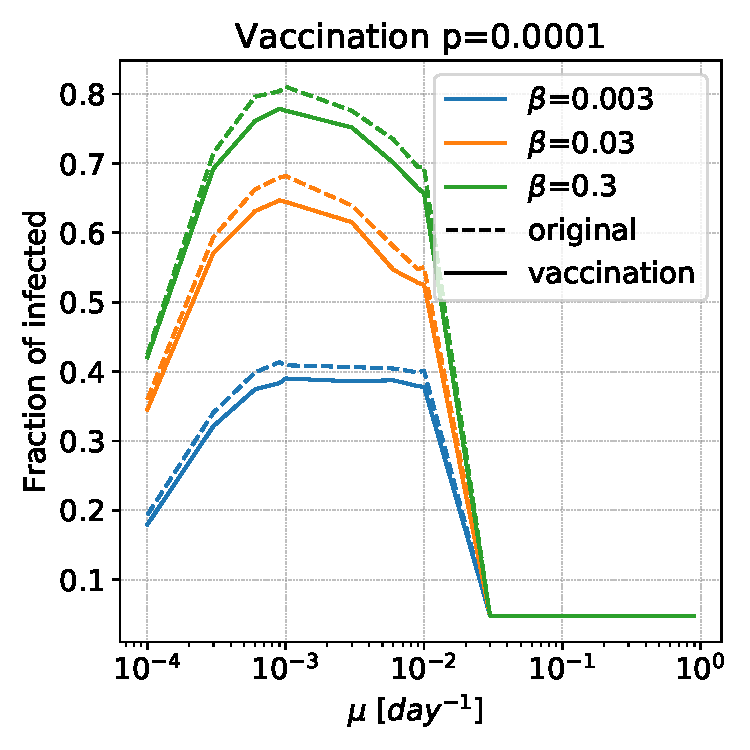
\includegraphics[scale=0.30]{./Figure/Simulations/SIR_vax/remove_0001.pdf}
\caption{}
\end{subfigure}
\begin{subfigure}[t]{0.32\textwidth}
\centering
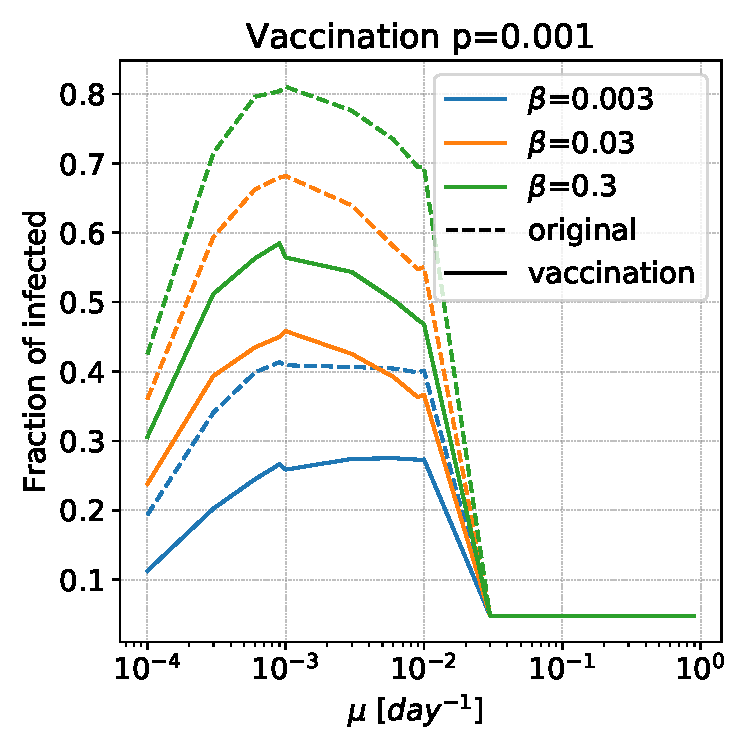
\includegraphics[scale=0.30]{./Figure/Simulations/SIR_vax/remove_001.pdf}
\caption{}
\end{subfigure}
\begin{subfigure}[t]{0.32\textwidth}
 \centering
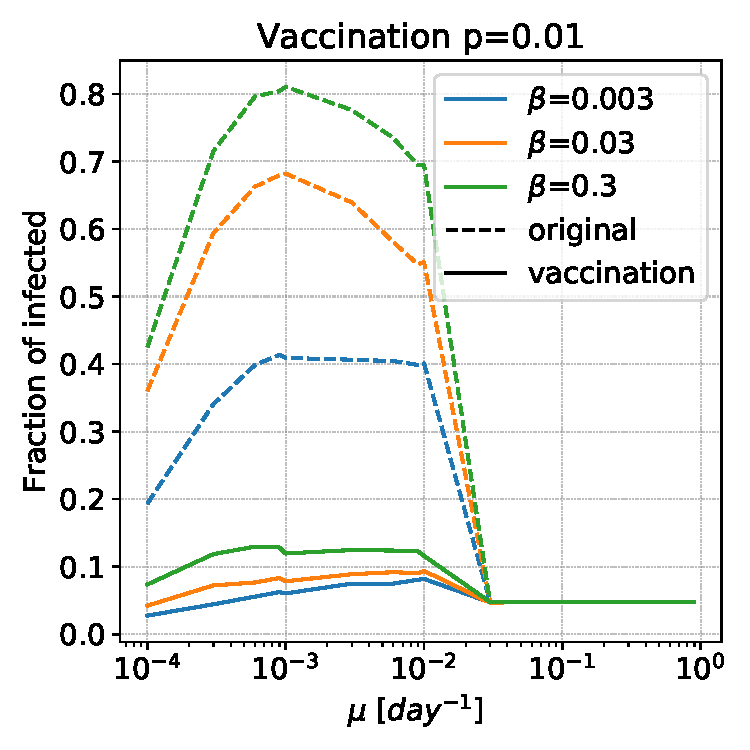
\includegraphics[scale=0.30]{./Figure/Simulations/SIR_vax/remove_01.pdf}
\caption{}
\end{subfigure}

\begin{subfigure}[t]{0.32\textwidth}
\centering
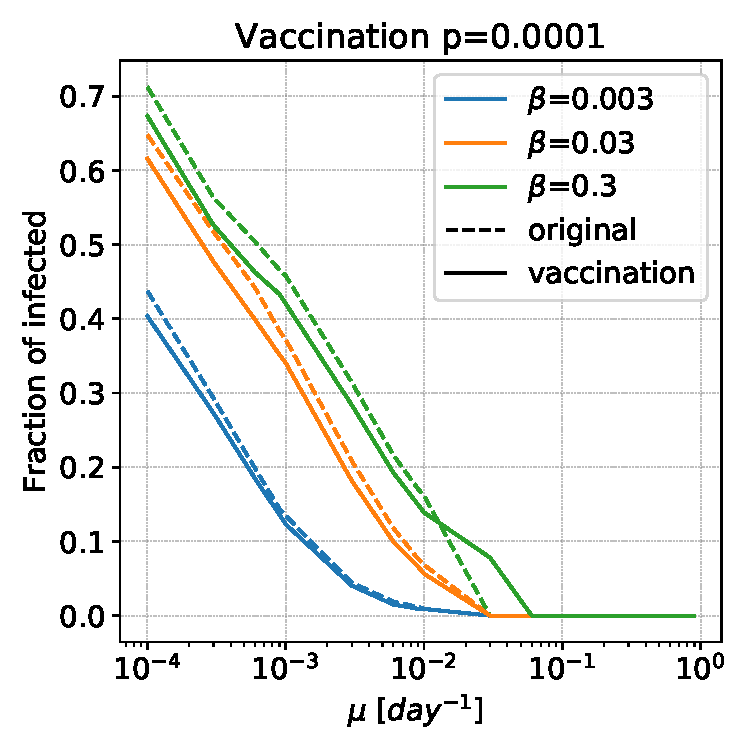
\includegraphics[scale=0.30]{./Figure/Simulations/SIS_vax/remove_0001.pdf}
\caption{}
\end{subfigure}
\begin{subfigure}[t]{0.32\textwidth}
\centering
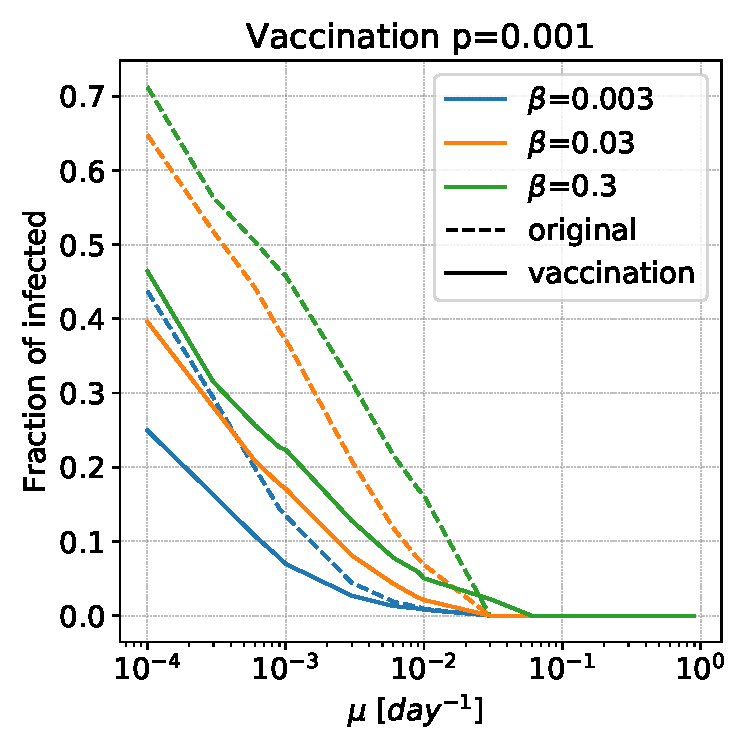
\includegraphics[scale=0.30]{./Figure/Simulations/SIS_vax/remove_001.pdf}
\caption{}
\end{subfigure}
\begin{subfigure}[t]{0.32\textwidth}
 \centering
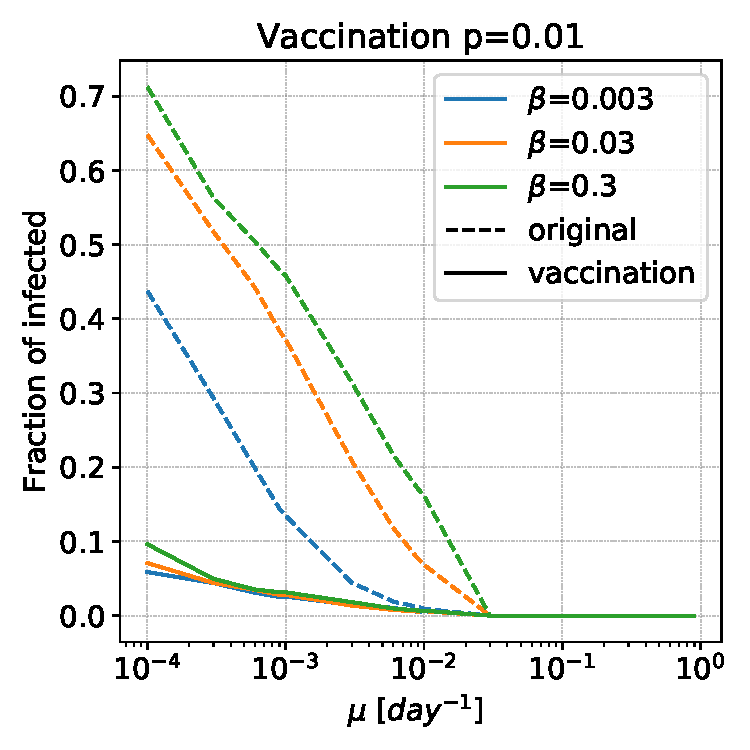
\includegraphics[scale=0.30]{./Figure/Simulations/SIS_vax/remove_01.pdf}
\caption{}
\end{subfigure}
\caption{Results for the vaccination strategies implemented with an underlying SIR model (Fig. A-C) and SIS model (Fig. D-F) on the temporal network. From left to right, the probability of each node to be vaccinated and hence obtain immunity at every time iteration is progressively higher, as labeled. Notice the $x$-axis is in logarithmic scale.}
\label{time_sims}
\end{figure*}

Once again, we compare a SIR and SIS model: in the former, a vaccinated node is just labeled as recovered (although in a different category, so that it can be distinguished from the recovered who did get the disease), in the latter is put in a group created \emph{ad hoc} for the same statistical purposes.

With the labeling tricks just mentioned, we can estimate with precision the \emph{fraction of infected} that we obtain at each combination of parameters (this is $r_{\infty}$ for SIR and $i_{\infty}$ for SIS), meaning the fraction of nodes who at some point in the time span considered contracted a disease whose epidemiologic description is coherent with the parameters themselves. 

These values appear to be significantly impacted by the vaccination policies, even for the smallest values of probability. Differently from the aggregated static network, in this case we notice a phase transition, in correspondence with the values of $\mu$ already pointed out in the previous grid search. Here we have a sudden change in behaviour that is fairly independent from the contagion rate $\beta$ and equally located in all cases, which makes it reasonable to think it could depend on the structure of the network rather than on the model or the specifics of the simulations performed on it.

What we can say, ultimately, is that it appears that the time dimension, with its intrinsic complexity, enriches the scenario and becomes a game-changing factor in effectiveness of vaccination. A proper vaccination schedule, if timed efficiently with the spreading dynamics of a certain disease in a given network, may reduce contamination up to $40\%$, even in very sparse communities such as the one made object of study.


%%%%%%%%%%%%%%%%%%%%%%%%%%%%%%%%%
%%%%%%% RRM AND EXTRA
%%%%%%%%%%%%%%%%%%%%%%%%%%%%%%%%%
\subsection{Manipulative analysis on temporal network}
\subsubsection*{Random reference models}
To compare our data with null models, we created two \emph{Randomized Reference Models} (RRMs):
\begin{itemize}
    \item a random reference model $RRM_1$ is created by shuffling at random the node list, altering the interactions but preserving the time flow at which they are supposed to happen;
    
    \item a random reference model $RRM_2$ is instead obtained by keeping the node lists consistent and shuffling the time intervals, hence breaking causality.
\end{itemize}

The idea behind these choices is that we want to compare our model with ones in which either the spatial or the temporal dimension have been deeply altered, reshaping the networks that happen to be built upon them.

To begin with, we display the topology and activations of the RRM models, comparing them with the original temporal network sequence.

\begin{figure}[H]
\begin{subfigure}[t]{0.24\textwidth}
\centering
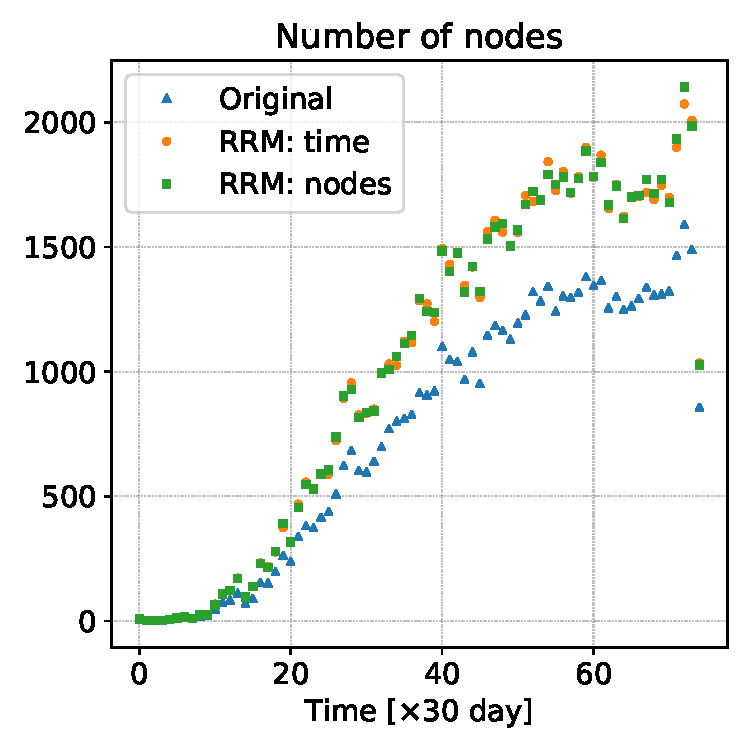
\includegraphics[width=\textwidth]{./Figure/Simulations/Number_nodes.pdf}
\caption{Active nodes at iteration}
\end{subfigure}
\begin{subfigure}[t]{0.24\textwidth}
 \centering
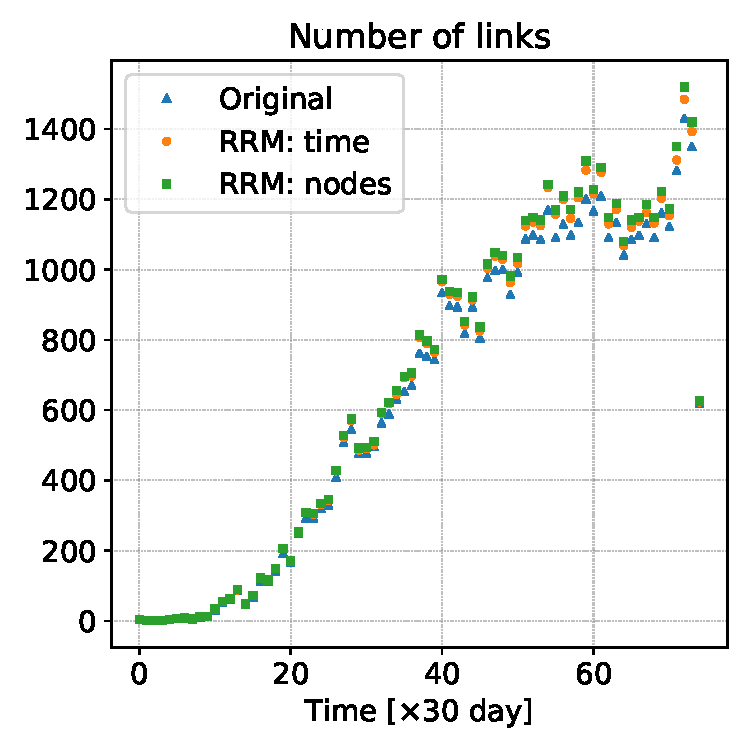
\includegraphics[width=\textwidth]{./Figure/Simulations/Number_edges.pdf}
\caption{Active links at iteration}
\end{subfigure}
\caption{Comparisons between the original time network sequence and the random reference models created to compare the simulations.}
\end{figure}

The node and link distributions are closely followed by both models, but the topology still is quantitatively modified, especially in the number of nodes.
\begin{figure}[htp]
\centering
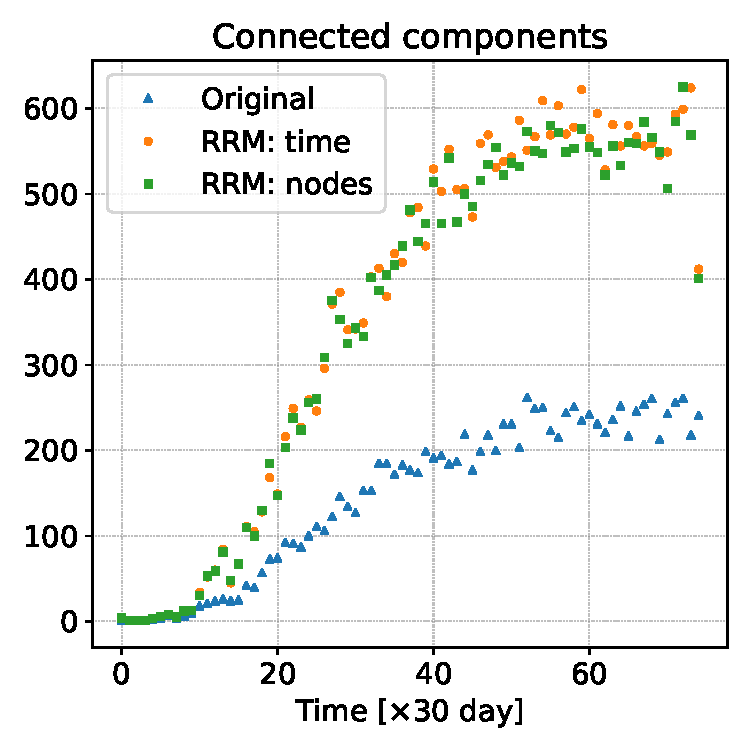
\includegraphics[scale=0.3]{./Figure/Simulations/connected_components.pdf}
\caption{Comparison between the number of connected components in the original time sequence and in the two mentioned RRMs.}
\end{figure}

If we consider the number of connected components, we noticed how the RRMs show an even greater sparsity than our initial time sequence. This is a foreseeable effect, as the breaking of time sequentiality alters the innate pair structure of the community, increasing randomness. This will likely represent an obstacle toward a profitable simulation.

This is, indeed, what happens when we run simulations on the RRM networks under the exact same conditions as the ones performed before.

\begin{figure}[H]
\begin{subfigure}[t]{0.24\textwidth}
\centering
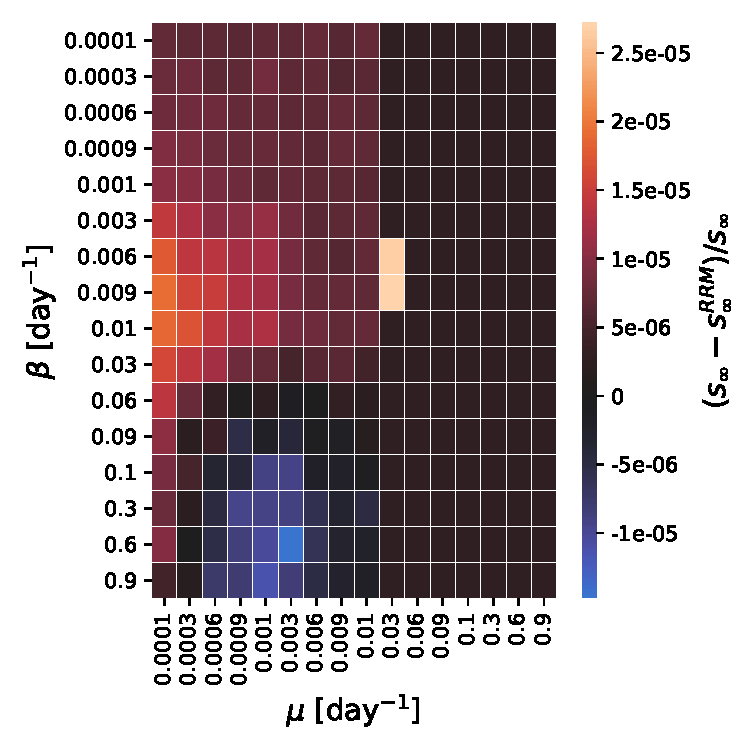
\includegraphics[scale=0.32]{./Figure/Simulations/SIR_temporal_RRM_nodes_96848_diff.pdf}
\caption{SIR; $RRM_1$}
\end{subfigure}
\begin{subfigure}[t]{0.24\textwidth}
 \centering
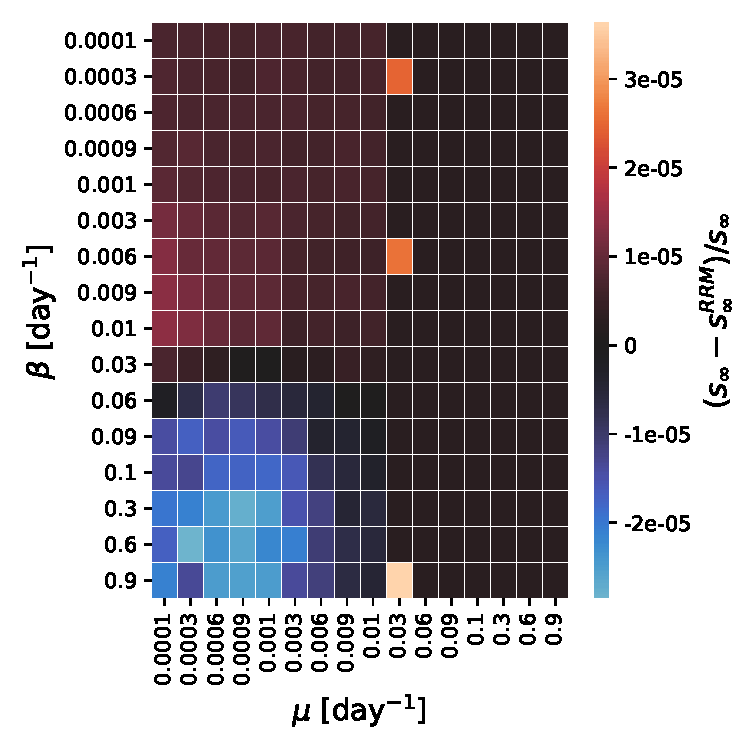
\includegraphics[scale=0.32]{./Figure/Simulations/SIR_temporal_RRM_time_19836_diff.pdf}
\caption{SIR; $RRM_2$}
\end{subfigure}

\begin{subfigure}[t]{0.24\textwidth}
\centering
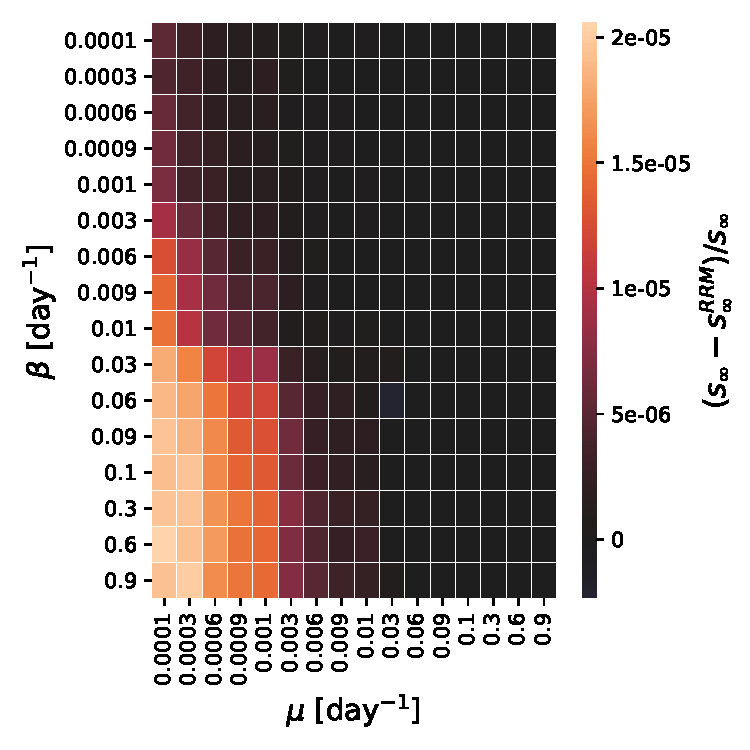
\includegraphics[scale=0.32]{./Figure/Simulations/SIS_temporal_RRM_nodes_26593_diff.pdf}
\caption{SIS; $RRM_1$}
\end{subfigure}
\begin{subfigure}[t]{0.24\textwidth}
 \centering
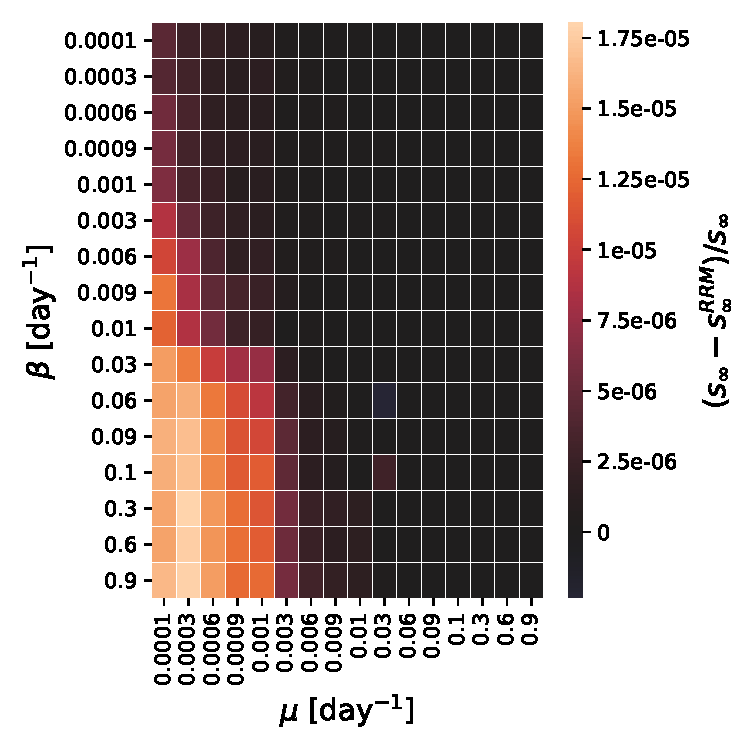
\includegraphics[scale=0.32]{./Figure/Simulations/SIS_temporal_RRM_time_65839_diff.pdf}
\caption{SIS; $RRM_2$}
\end{subfigure}

\caption{Heatmaps showing the residuals between each RRM and the original sequence with both a SIR and a SIS model; notice from the color bar that the scale is extremely fine, meaning the differences between the models are basically negligible.}
\end{figure}

While the patterns obtained are somewhat noteworthy, we should immediately notice that the scale is extremely fine in values: since we are considering relative residuals, the fact that they all consistently lie in the order of magnitude of $10^{-5}$ is a good indicator that no substantial information can be extracted from the RRM models.

On a general note, the SIR model still appears to be the one with greater variability in the parameters, but these effects could still be due to statistical fluctuations.


\subsubsection*{Removal of bystanders}
As a final attempt at obtaining a more permeable network, we implement the removal of what we define \emph{bystanders}, those people -- men or women, we do not distinguish -- that undergo less than 5 activation in the time period considered and therefore are the main responsible for the sparseness of our dataset (and, in reality, of Internet-mediated prostitution communities as a whole).

\begin{figure}[H]
\begin{subfigure}[t]{0.24\textwidth}
\centering
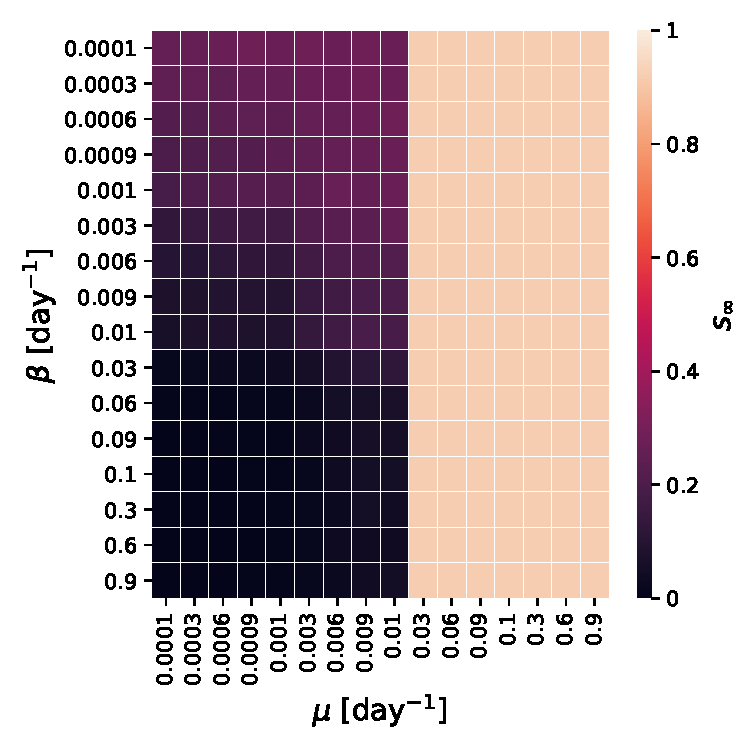
\includegraphics[scale=0.30
]{./Figure/Simulations/SIR_temporal_53706_rm5.pdf}
\caption{SIR, absolute values}
\end{subfigure}
\begin{subfigure}[t]{0.24\textwidth}
 \centering
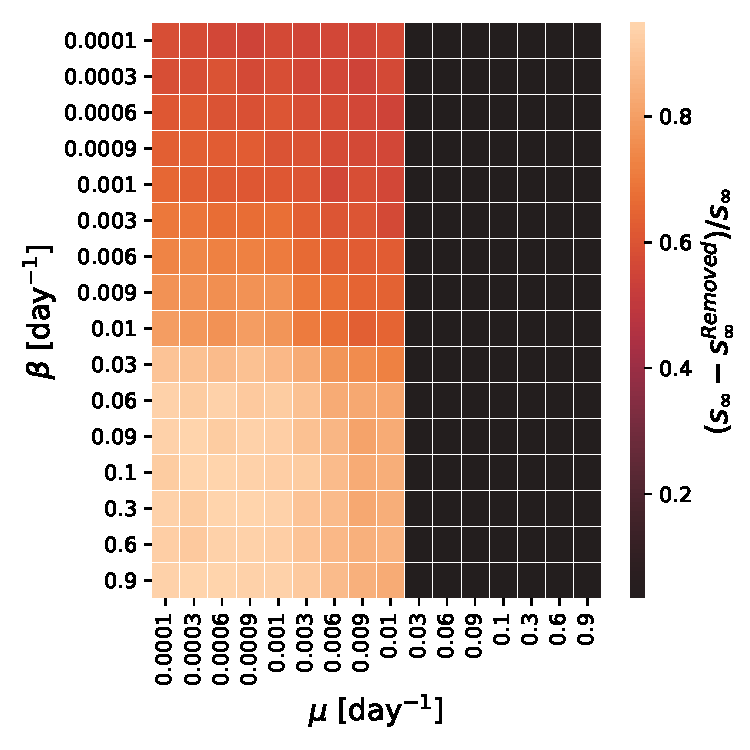
\includegraphics[scale=0.30]{./Figure/Simulations/SIR_temporal_53706_rm5_diff.pdf}
\caption{SIR, relative residuals}
\end{subfigure}

\begin{subfigure}[t]{0.24\textwidth}
\centering
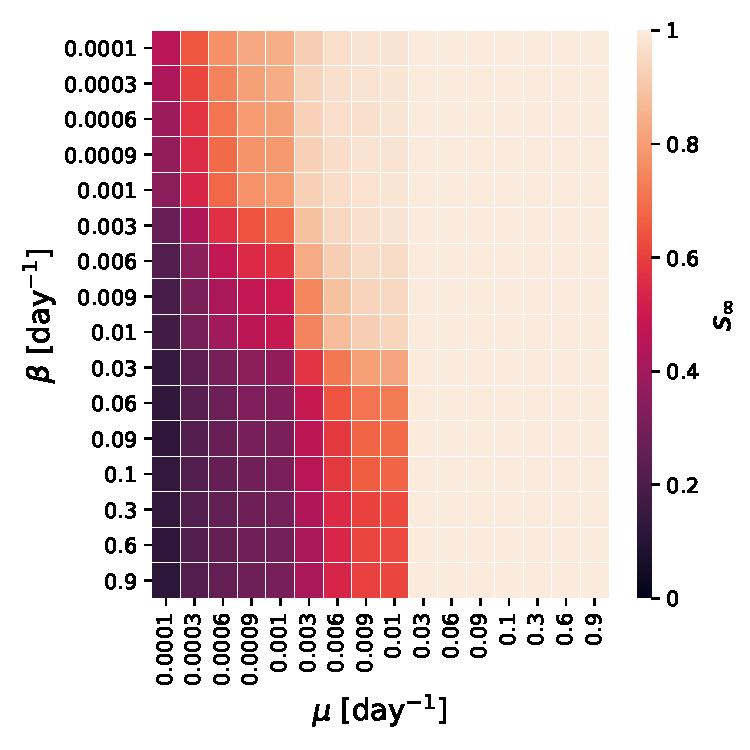
\includegraphics[scale=0.30]{./Figure/Simulations/SIS_temporal_30330_rm5.pdf}
\caption{SIS, absolute values}
\end{subfigure}
\begin{subfigure}[t]{0.24\textwidth}
 \centering
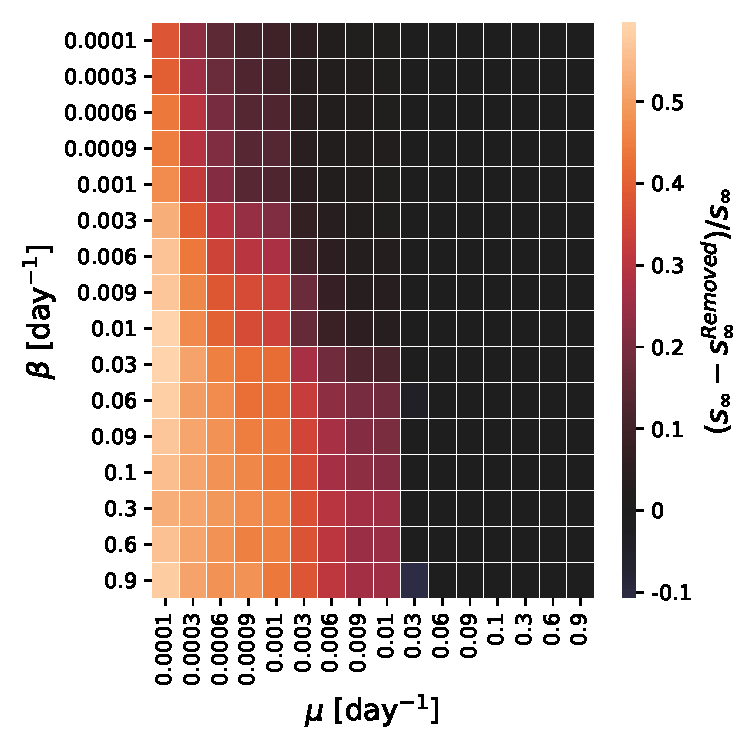
\includegraphics[scale=0.30]{./Figure/Simulations/SIS_temporal_30330_rm5_diff.pdf}
\caption{SIS, relative residuals}
\end{subfigure}

\caption{Heatmaps showing the fraction $s_{\infty}$ of susceptibles at equilibrium for each combination of parameters $\beta$ and $\mu$ in the case where the nodes with less that 5 total activations have been removed from the network. The ones on the left show absolute values, while those on the right hand side relative residuals with the original model.}
\end{figure}

Once again, we perform simulations in the form of a grid search through a SIR and a SIS models. This will help us evaluate if there are macroscopic differences in the outbreak patterns obtained like so.

The heatmaps show the relative differences with our original time network sequence. Clearly, at each iteration, the amount was already normalized in itself with the total number of nodes present at that iteration, in order to obtain a fractional value; periodicity has been defined as previously.

Not surprisingly, the relative differences increase in those regions of the parameter space where the values were the lowest in the original model. This means that our node removal policy was effective: we observe spreading where there was not previously, so we managed to obtain a community whose sparsity is not its dominant feature. For other choices of hyperparameters, nothing peculiar happens and the phase transition is still neatly visible; the general trend appears to be preserved in both models. 


%%%%%%%%%%%%%%%%%%%%%%%%%%%%%%%%%
%%%%%%% DISCUSSION & CONCLUSION
%%%%%%%%%%%%%%%%%%%%%%%%%%%%%%%%%
\section{Discussion}
As a general, introductory consideration, we point out that we obtained drastically different results between static and dynamic networks. The time dimension proved to be an enriching feature in our analysis and it in a way modulated the extreme sparsity of the activations in the community.

The first hint of this complex structure was found already when simulating a SIR or SIS model onto the network. On the one side, having the time information at disposal made it possible to find new ways to increase the realism of the simulations themselves; on the other side, a different structure altogether seemed to emerge from the temporal network, with the display of a sort of phase transition.

This is the most surprising result of the whole analysis: the SIR model has a sharp critical recovery time after which no spreading ever seems to occur. In practice. this means that those diseases that can be described suitably by this model in that parameter range will need not be taken care of directly, because it appears impossible for them to become endemic in this kind of communities anyways.

The temporal network also appears to be more prone to vaccination strategies, which in general scored an increased effectiveness. This happens mainly because having a time dimension allows for new, more efficient vaccination strategies to be implemented, with greater probability of an extended targeting even in a sparse community. As a practical application, this enforces the fact that a long-term vaccination program is likely to be more effective and, interestingly, its increased effectiveness is dependent on the network the vaccine is spread among, not strictly on the disease it is meant to fight against.

The comparison with RRM models proved to be rather uninformative: neither healed the sparseness of the original network and, as a matter of fact, the relative differences obtained in the simulations are so small they basically are statistical fluctuations. This, in turn, could mean a positive indication of the soundness of our previous analysis.

Finally, a quick note on the bystander removal. While it is true that this operation deeply modifies our network and it hence diverts our analysis, it gave precious indication of a way to make our community more permeable to disease spreading. This will hopefully result in the possibility of more interesting further studies at the vaccination level.


\section{Conclusions}
Our analysis made it clear that the time dimension broadens the scenario when an epidemiologic point of view is chosen to study spreading and vaccination techniques in a dynamical community of people.

The time information is indeed a remarkably useful description tool, but it also opened new ways to deal with outbreak simulations and preventive containment strategies. 

It should be noted, however, that the network obtained with the data at disposal was characterized by extreme sparsity, which has indeed influenced our results in several circumstances.

\newpage
\bibliographystyle{IEEEtran}
\addcontentsline{toc}{chapter}{Bibliography}
{\footnotesize
\bibliography{bibliography.bib}
}



\end{document}